% Number 241
% CVPMG Units
% Football players running at each other: graphical version
% JG

% Watermark
\AddToShipoutPicture*{\BackgroundPic}

\addtocounter {ProbNum} {1}

%\begin{floatingfigure}[r]{.4\textwidth}
%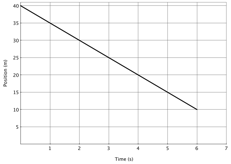
\includegraphics[scale=1]{/Users/jgates/desktop/latex/pics/flipper.png}
%\end{floatingfigure}
 
{\bf \Large{\arabic{ProbNum}}} A running back carries the football down the field, running ${5.6~\tfrac{m}{s}}$.  The slower safety (running speed: ${4.5~\tfrac{m}{s}}$) runs towards him and tries to tackle him. They begin 22 meters apart and run straight at each other.  
%\begin{center} 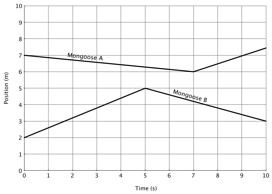
\includegraphics[scale=1]{/Users/jgates/desktop/latex/pics/mongooses.png}
%\end{center}

\bigskip

How far did the running back go before being tackled, and how much time elapsed before he was tackled? Use graphical problem solving.
 
\vfill

\newpage
